\documentclass[a4paper,slidestop,xcolor=pst,blue]{beamer}

\usepackage{beamerthemesplit}
\usepackage[utf8]{inputenc}
\usepackage[spanish]{babel}
\usepackage{graphicx}
\usepackage{pstricks} % PSTricks package
\usepackage{setspace}
\usepackage{multirow}
\usepackage{listings}
\usepackage{pgfpages}
\usepackage{hyperref}
\usepackage{etoolbox}
\usepackage{epstopdf}

\makeatletter
\patchcmd{\beamer@sectionintoc}{\vskip1.5em}{\vskip0.5em}{}{}
\makeatother

\setbeamercovered{dynamic}
\setcounter{tocdepth}{2}
\setbeamercolor{frametitle}{fg=black,bg=white}
\setbeamercolor{section in toc shaded}{fg=black}
\setbeamercolor{section in toc}{fg=red}
\setbeamercolor{subsection in toc shaded}{fg=black}
\setbeamercolor{subsection in toc}{fg=red}
\setbeamerfont{section in toc}{size=\small}
\setbeamerfont{subsection in toc}{size=\small}
\setbeamertemplate{section in toc shaded}[default][99]
\setbeamertemplate{subsection in toc shaded}[default][99]

\AtBeginSection[]
{\begin{frame}[c]
  \frametitle{Índice}
	\tableofcontents[currentsection,
        sectionstyle=show/shaded,
        subsectionstyle=hide]
\end{frame}}

\AtBeginSubsection[]
{\begin{frame}[c]
	\frametitle{Índice}
	\tableofcontents[
  		currentsection,
  		sectionstyle=shaded/shaded,
  		currentsubsection,
  		subsectionstyle=show/shaded/hide
		]
\end{frame}}

\setbeamercolor{frametitle}{fg=black,bg=white}

\setbeamertemplate{frametitle}{
	\begin{centering}
		\insertframetitle
		\par
	\end{centering}
}

\usetheme[secheader]{Boadilla} 

\title[Capa de Persistencia]{Capa de Persistencia}

\author[P. S{\'a}nchez]{\alert{Pablo S{\'a}nchez}}

\institute[IIE]{
		   Dpto. Ingenier{\'i}a Inform{\'a}tica y Electr{\'o}nica \\
		   Universidad de Cantabria \\
		   Santander (Cantabria, Espa{\~n}a) \\
		   \texttt{p.sanchez@unican.es}
}

\date{}

\begin{document}

%\begin{frame}[c]
%	\titlepage
%	\begin{columns}
%		\column{0.50\linewidth}
%			\centering
%    		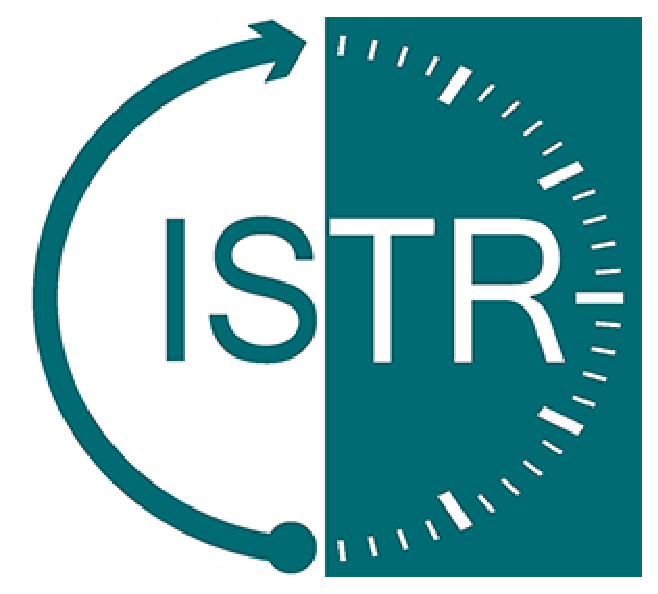
\includegraphics[width=.28\textwidth,keepaspectratio=true]{images/istr.eps}
%		\column{0.50\linewidth}
%			\centering
%			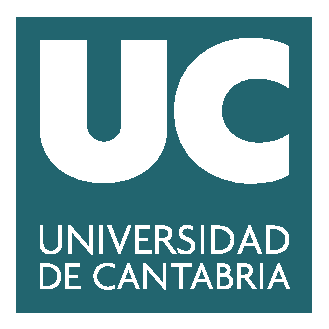
\includegraphics[width=.25\textwidth,keepaspectratio=true]{images/uc.eps}
%	\end{columns}
%\end{frame}
%
%\begin{frame}[c]
%    \frametitle{\alert{Advertencia}}
%    \begin{center}
%        Todo el material contenido en este documento no constituye en modo alguno una obra de referencia o apuntes oficiales mediante el cual se puedan preparar las pruebas evaluables necesarias para superar la asignatura. \ \\
%        \ \\
%        Este documento contiene exclusivamente una serie de diapositivas cuyo objetivo es servir de complemento visual a las actividades realizadas en el aula para la transmisi{\'o}n del contenido sobre el cual versar{\'a}n las mencionadas pruebas evaluables.  \ \\
%        \ \\
%        Dicho de forma m{\'a}s clara, \alert{estas transparencias no son apuntes y su objetivo no es servir para que el alumno pueda preparar la asignatura.}
%    \end{center}
%\end{frame}

%\section{Introducción}
%
%\begin{frame}
%    \frametitle{Capa de Persistencia}
%    \only<1|handout:2>{
%        \rput[lt](0,0){
%            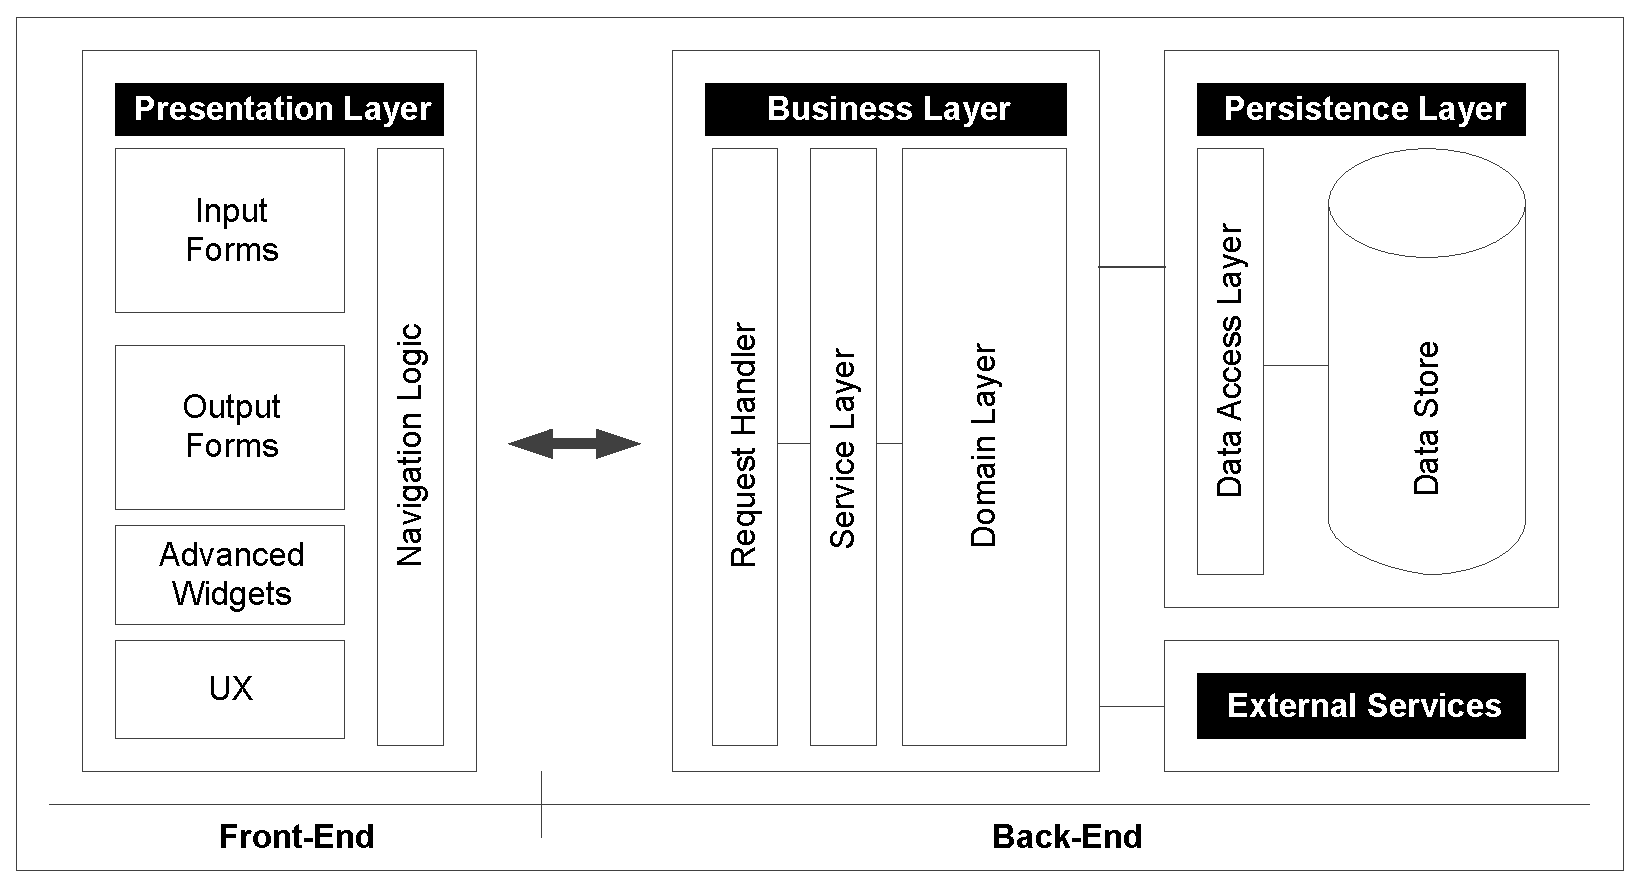
\includegraphics[width=\linewidth]{images/intro/enterpriseArchitectures00.eps}
%        }
%    }
%    \only<2|handout:2>{
%        \rput[lt](0,0){
%            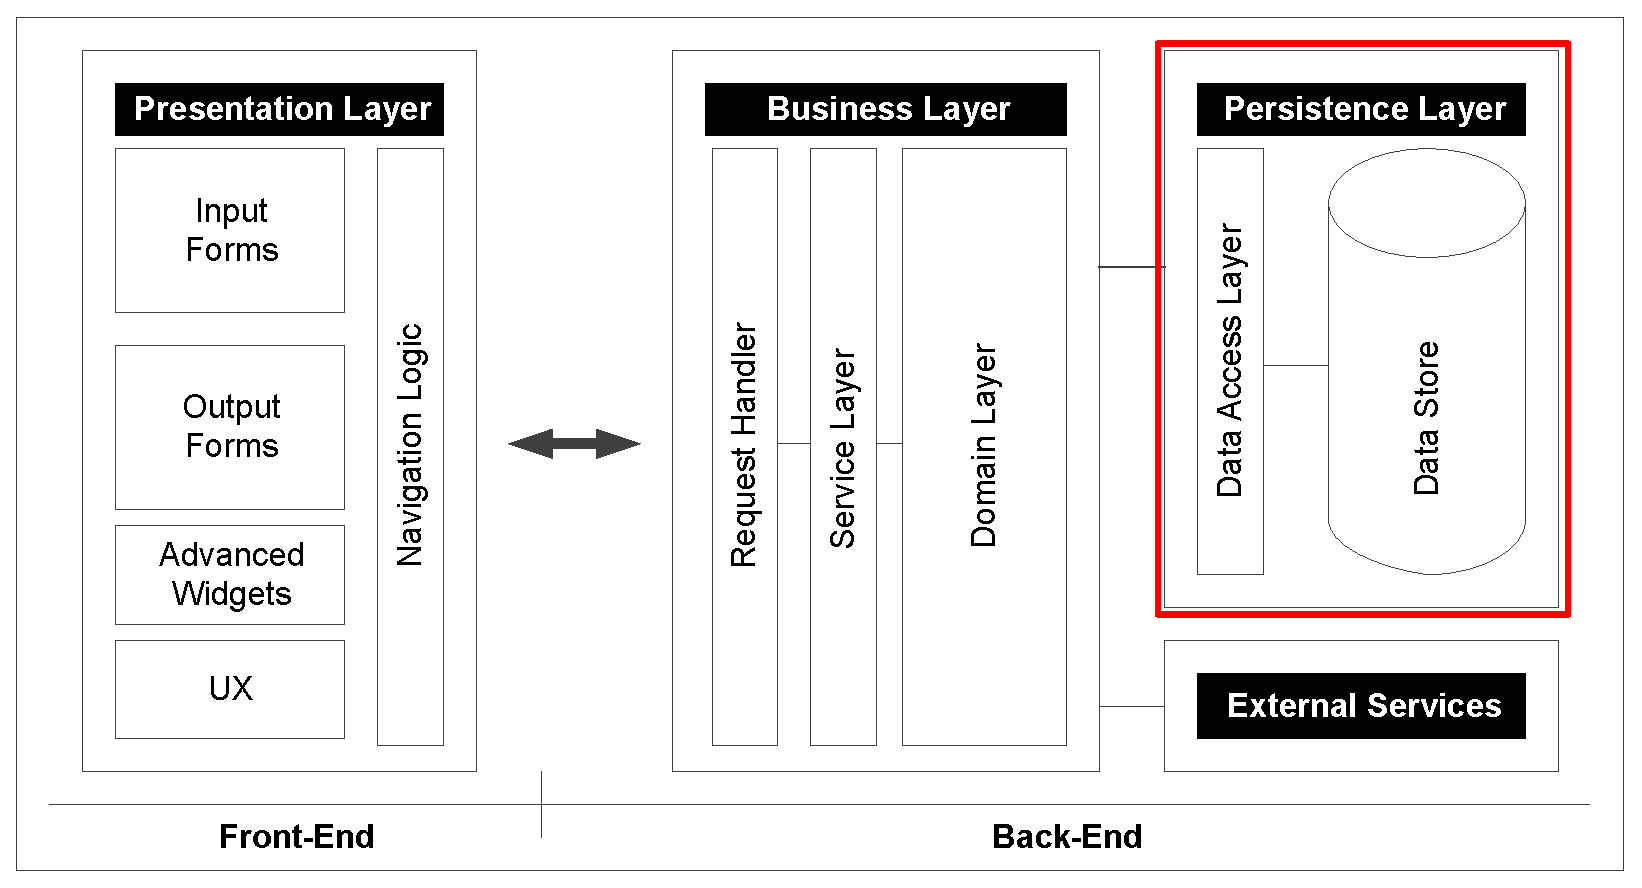
\includegraphics[width=\linewidth]{images/intro/enterpriseArchitectures01.eps}
%        }
%    }
%\end{frame}
%
%\begin{frame}[c]
%	\frametitle{Responsabilidades de la Capa de Persistencia}
%	\begin{enumerate}[<+->]
%        \item Almacenar los datos de manera no volátil.
%        \item Recuperar datos del almacén persistente.
%        \item Asegurar la disponibilidad de los datos.
%        \item Controlar la integridad de los datos.
%        \item Asegurar un acceso eficiente a los datos.
%	\end{enumerate}
%\end{frame}
%
%\begin{frame}[c]
%    \frametitle{Objetivos del Tema}
%    \begin{enumerate}[<+->]
%         \item Comprender en profundidad cuáles son las responsabilidades de la capa de persistencia.
%         \item Comprender el objetivo de los puentes objeto-(relacional).
%         \item Comprender los principios de los patrones de persistencia estructurales.
%         \item Comprender el funcionamiento de los patrones de acceso a datos.
%         \item Ser capaz de utilizar \emph{JPA} para generar esquemas relacionales.
%         \item Ser capaz de utilizar repositorios \emph{Spring} para acceder a datos.
%    \end{enumerate}
%\end{frame}
%
%\begin{frame}[c]
%    \frametitle{Bibliografía}
%    \begin{thebibliography}{1}
%
%        \bibitem[Fowler, 2002]{Fowler2002}
%        Fowler, M. (2002).
%        \newblock {\em {Patterns of Enterprise Application Architecture}}.
%        \newblock Addison-Wesley.
%
%        \bibitem[Esposito and Saltarello, 2014]{Esposito2014}
%        Esposito, D. y Saltarello, A. (2014).
%        \newblock {\em {Microsoft .NET - Architecting Applications for the
%          Enterprise}}. 2ª Ed..
%        \newblock Microsoft Press
%
%        \bibitem[Bauer, 2015]{Bauer2015}
%        Bauer, C., King. G. y Gregory G. (2015).
%        \newblock {\em {Java Persistence with Hibernate}}. 2ª Ed.
%        \newblock Manning
%
%        %% Spring Data
%
%    \end{thebibliography}
%\end{frame}
%
%%\begin{frame}[c]
%%    \frametitle{Tecnologías de Persistencia}
%%    \begin{description}[<+->]
%%        \item[Relacional] Madurez, robustez y propiedades ACID.
%%        \item[NoSQL] Escalabilidad y rendimiento sacrificando ACID.
%%        \item[XML/JSON] Simplicidad.
%%    \end{description}
%%\end{frame}
%
%\section{Puentes de Persistencia de Objetos}
%
%\subsection{Impedancia Objeto - Persistencia}
%
%\begin{frame}[c]
%    \frametitle{Impedancia Objeto - (Relacional)}
%    \begin{block}{Impedancia Objetual}
%    La \emph{impedancia objetual} se refiere al desacoplamiento que puede existir en los conceptos del paradigma orientado a objetos y el paradigma utilizado por el almacén de persistencia.
%    \end{block}
%\end{frame}
%
%\begin{frame}[c]
%    \frametitle{Impedancia Objeto - Relacional}
%    \begin{center}
%        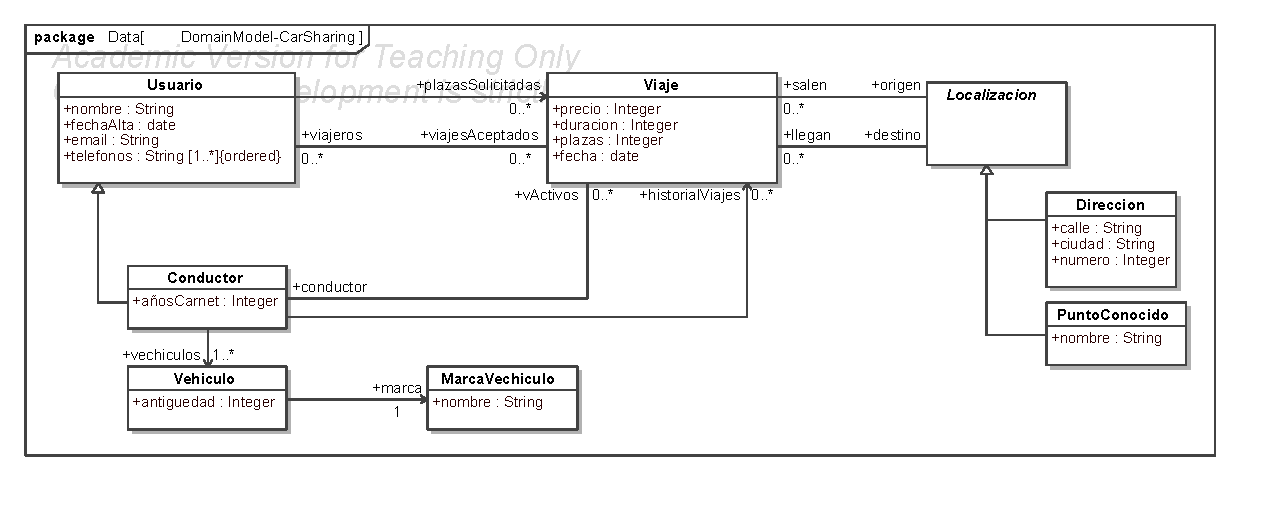
\includegraphics[width=\linewidth]{images/ooMismatch/ooMismatch00.eps}
%    \end{center}
%\end{frame}
%
%\begin{frame}[c]
%    \frametitle{Impedancia Objeto - Relacional}
%    \begin{center}
%        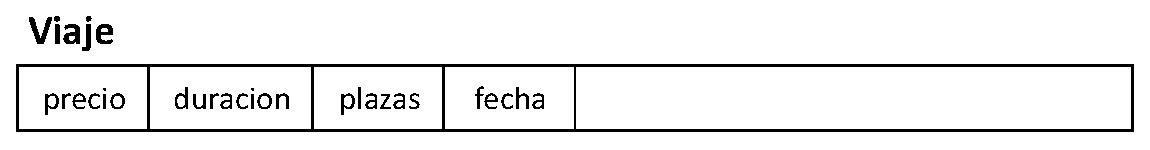
\includegraphics[width=0.8\linewidth]{images/ooMismatch/ooMismatch01.eps}
%    \end{center}
%\end{frame}
%
%\begin{frame}[c]
%    \frametitle{Impedancia OR: Claves Primarias}
%    \begin{center}
%        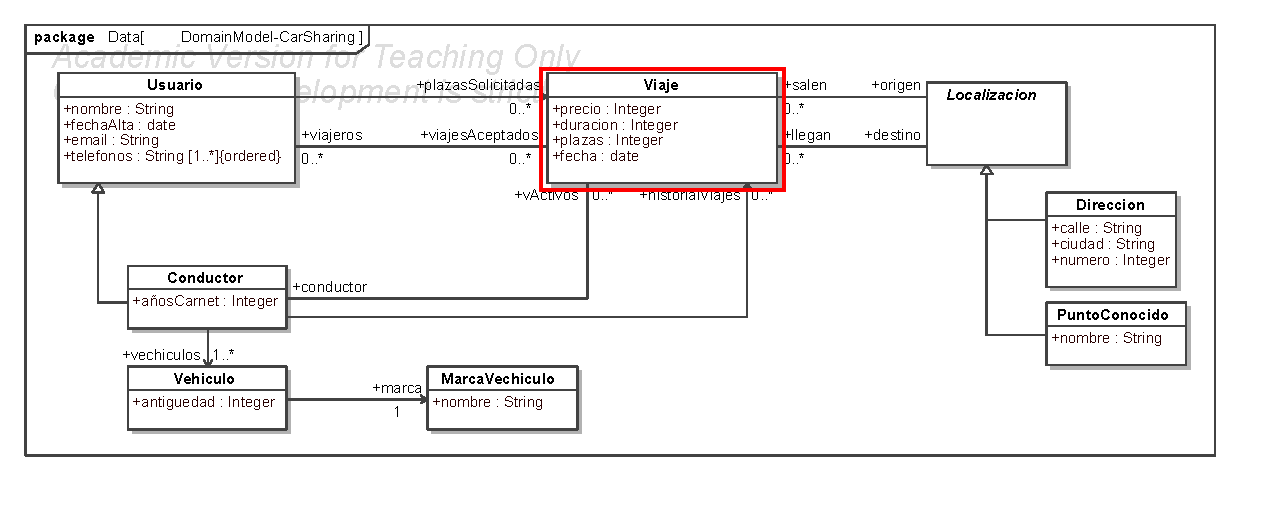
\includegraphics[width=\linewidth]{images/ooMismatch/ooMismatch09.eps}
%    \end{center}
%\end{frame}
%
%\begin{frame}[c]
%    \frametitle{Impedancia OR: Atributos Multivaluados}
%    \begin{center}
%        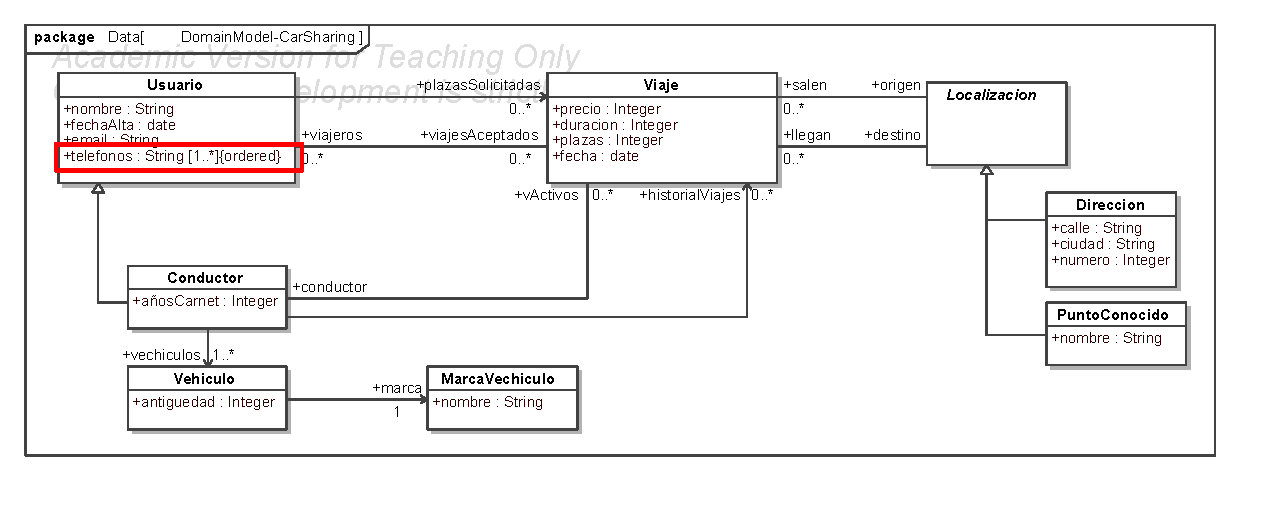
\includegraphics[width=\linewidth]{images/ooMismatch/ooMismatch02.eps}
%    \end{center}
%\end{frame}
%
%\begin{frame}[c]
%    \frametitle{Impedancia OR: Atributos Multivaluados}
%    \begin{center}
%        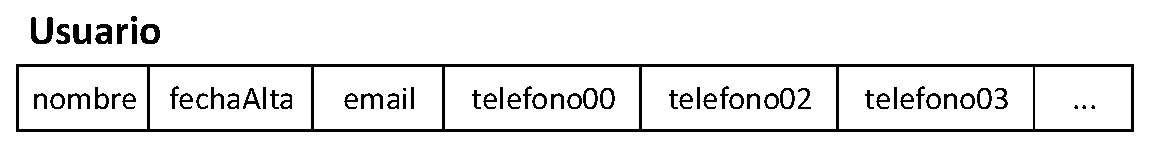
\includegraphics[width=0.8\linewidth]{images/ooMismatch/ooMismatch03.eps}
%    \end{center}
%\end{frame}
%
%\begin{frame}[c]
%    \frametitle{Impedancia OR: Herencia}
%    \begin{center}
%        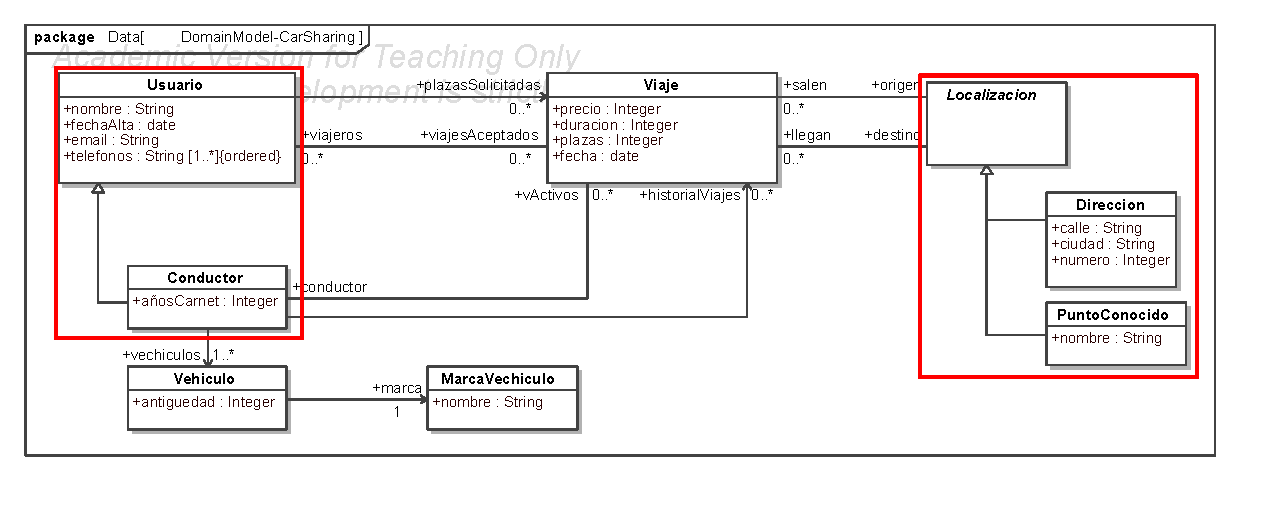
\includegraphics[width=\linewidth]{images/ooMismatch/ooMismatch04.eps}
%    \end{center}
%\end{frame}
%
%\begin{frame}[c]
%    \frametitle{Impedancia OR: Navegabilidad Asociaciones}
%    \begin{center}
%        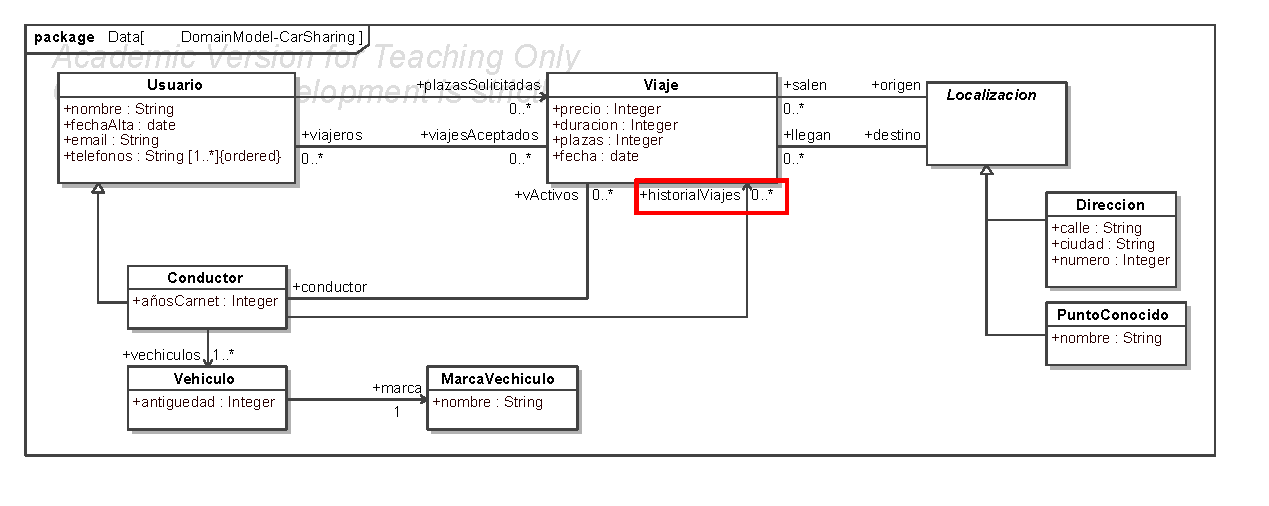
\includegraphics[width=\linewidth]{images/ooMismatch/ooMismatch05.eps}
%    \end{center}
%\end{frame}
%
%\begin{frame}[c]
%    \frametitle{Impedancia OR: Navegabilidad Asociaciones}
%    \begin{center}
%        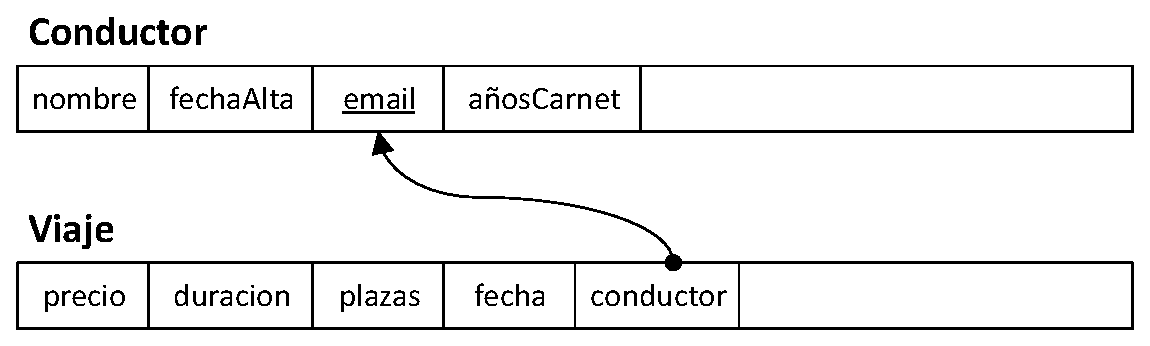
\includegraphics[width=0.8\linewidth]{images/ooMismatch/ooMismatch06.eps}
%    \end{center}
%\end{frame}
%
%\begin{frame}[c]
%    \frametitle{Impedancia OR: Asociaciones Muchos a Muchos}
%    \begin{center}
%        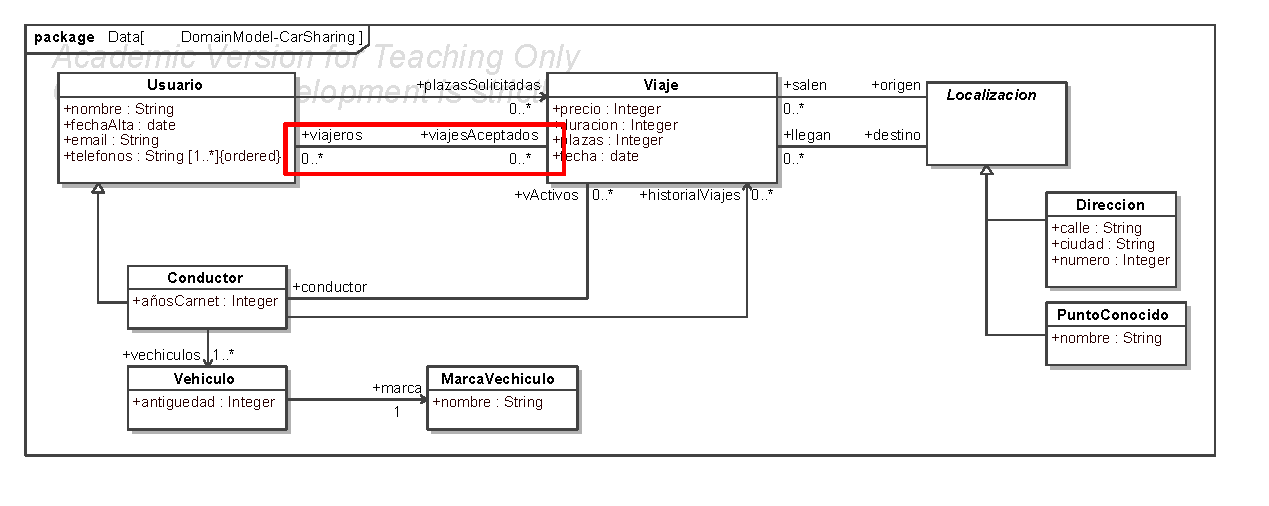
\includegraphics[width=\linewidth]{images/ooMismatch/ooMismatch07.eps}
%    \end{center}
%\end{frame}
%
%\begin{frame}[c]
%    \frametitle{Impedancia OR: Asociaciones Muchos a Muchos}
%    \begin{center}
%        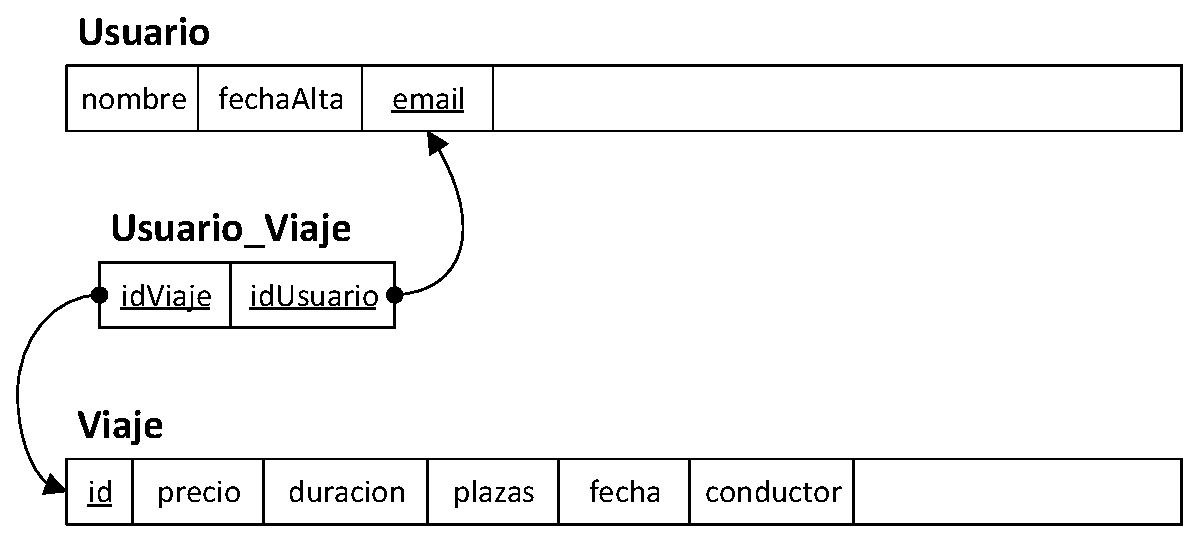
\includegraphics[width=0.8\linewidth]{images/ooMismatch/ooMismatch08.eps}
%    \end{center}
%\end{frame}
%
%\begin{frame}[c]
%    \frametitle{Impedancia OR: Granularidad}
%    \begin{center}
%        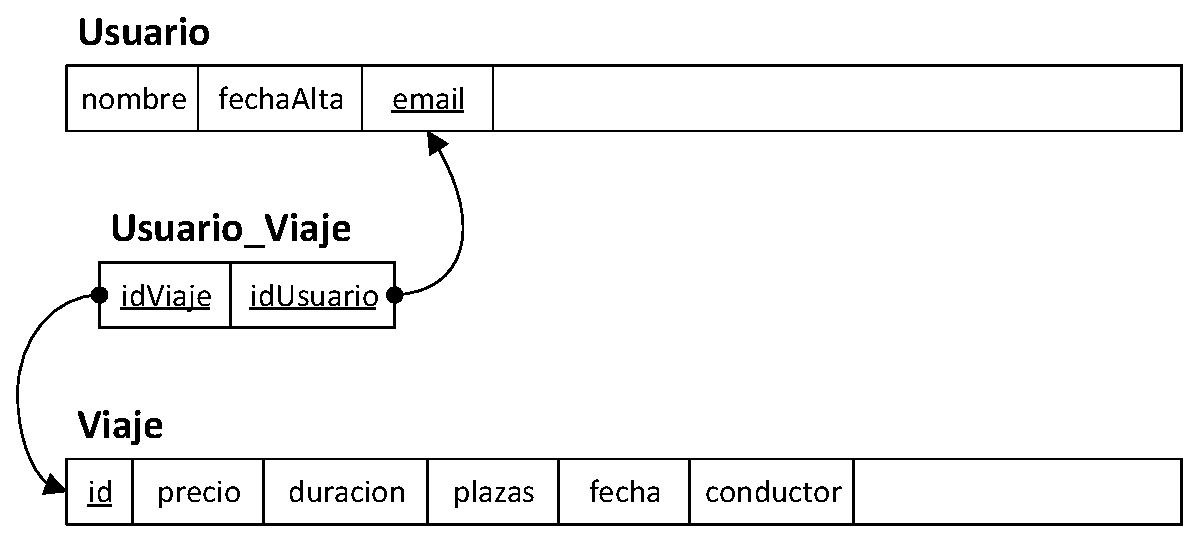
\includegraphics[width=0.8\linewidth]{images/ooMismatch/ooMismatch08.eps}
%    \end{center}
%\end{frame}
%
%\subsection{Puentes Objeto-(Relacional)}
%
%\begin{frame}
%    \frametitle{Puentes de Persistencia de Objetos}
%    \only<1|handout:3>{
%        \rput[lt](0,0){
%            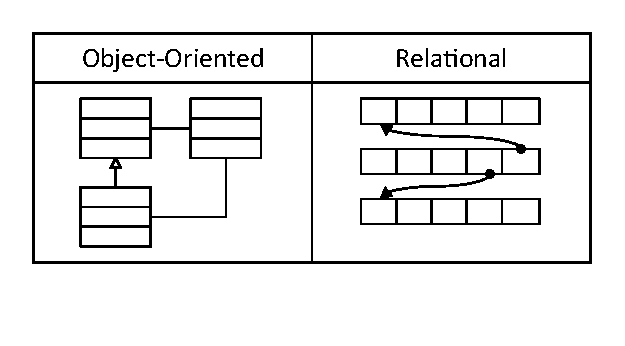
\includegraphics[width=\linewidth]{images/ooMismatch/orm00.eps}
%        }
%    }
%    \only<2|handout:3>{
%        \rput[lt](0,0){
%            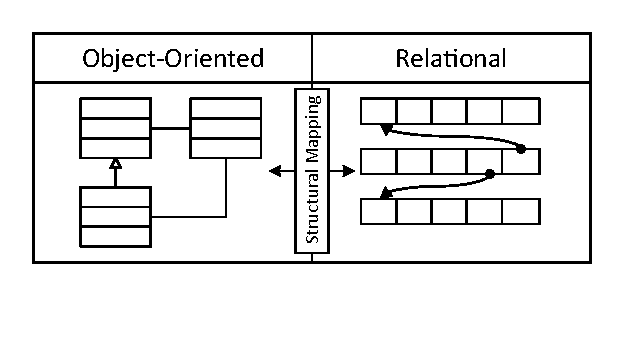
\includegraphics[width=\linewidth]{images/ooMismatch/orm01.eps}
%        }
%    }
%    \only<3|handout:3>{
%        \rput[lt](0,0){
%            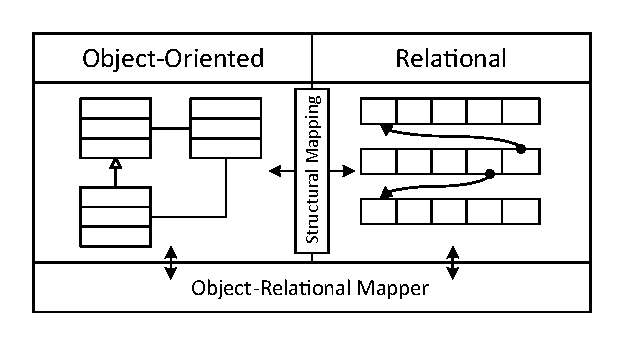
\includegraphics[width=\linewidth]{images/ooMismatch/orm02.eps}
%        }
%    }
%    \only<4|handout:3>{
%        \rput[lt](0,0){
%            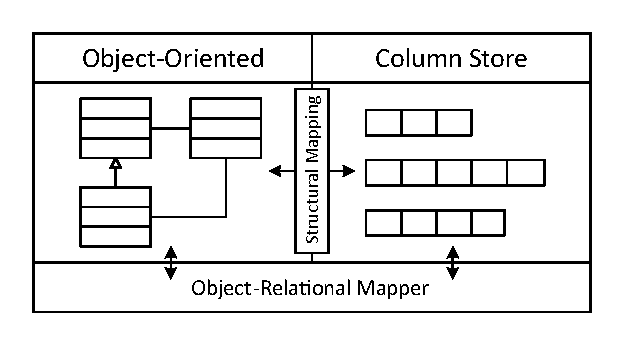
\includegraphics[width=\linewidth]{images/ooMismatch/orm03.eps}
%        }
%    }
%\end{frame}
%
%\section{Patrones Estructurales}
%
%\subsection{Class to Table}
%
%\begin{frame}[c]
%    \frametitle{Class to Table}
%    \begin{block}{Problema}
%        \begin{enumerate}
%            \item ¿Cómo transformo una clase a relacional?
%        \end{enumerate}
%    \end{block}
%    \uncover<2->{
%        \begin{block}{Solución}
%            Si la clase es una \emph{entidad}, no está afectada por herencia, y no tiene atributos multivaluados ni asociaciones con otras clases:
%            \begin{enumerate}
%                \item<3-> Crear una tabla con el mismo nombre de la clase.
%                \item<4-> Crear una columna en dicha tabla por cada atributo de la clase.
%                \item<5-> Asignar como tipo de la columna el tipo que corresponda a cada atributo.
%            \end{enumerate}
%        \end{block}
%    }
%\end{frame}
%
%\begin{frame}
%    \frametitle{Class to Table}
%    \rput[lt](3.5,0){
%            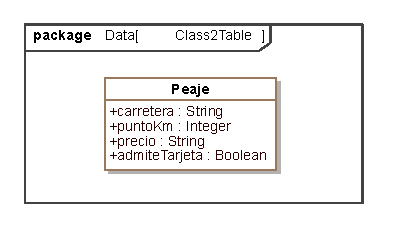
\includegraphics[width=0.50\linewidth]{images/structure/class2Table00.eps}
%    }
%    \only<2->{
%        \rput[lt](3,-4){
%                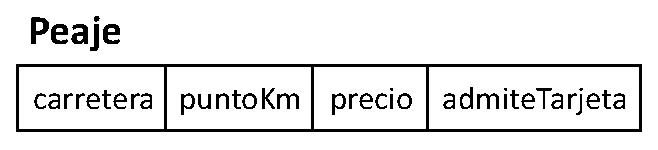
\includegraphics[width=0.50\linewidth]{images/structure/class2Table01.eps}
%        }
%    }
%\end{frame}
%
%\subsection{Identity Field}
%
%\begin{frame}[c]
%    \frametitle{Identity Field}
%    \begin{block}{Problema}
%        \begin{enumerate}
%            \item<1-> ¿Cómo consigo que cada objeto de una clase tenga asociada una clave primaria que pueda utilizar para almacenarlo en una tabla de una base de datos relacional?
%            \item<2-> ¿Cómo consigo mantener la correspondencia entre cada objeto de una clase y su correspondiente representación relacional cuando los objetos no tienen clave natural?
%        \end{enumerate}
%    \end{block}
%    \uncover<3->{
%        \begin{block}{Solución}
%            \begin{enumerate}
%                \item<4-> Incorporar un nuevo atributo, representando una clave artificial, para aquellos objetos que no poseen una clave natural, o cuya clave natural se considere inadecuada para el modelo relacional.
%                \item<5-> Para las claves artificiales, elegir una estrategia de generación.
%            \end{enumerate}
%        \end{block}
%    }
%    %% To be discussed:
%    %% - Natural vs Artifical Key
%    %% - Single vs Compound Key
%    %% - Key Type
%    %% - Table Unique vs Database Unique
%\end{frame}
%
%\begin{frame}[c]
%    \frametitle{Generación de Claves Artificales}
%    \begin{enumerate}
%        \item<1-> Columna autoincrementada
%            \begin{itemize}
%                \item<2-> Clave no disponible hasta finalizar la transacción.
%                \item<3-> Impide \emph{escrituras en batch}
%            \end{itemize}
%        \item<4-> Sequence
%            \begin{itemize}
%                \item<5-> No disponible en todos los gestores.
%            \end{itemize}
%        \item<6-> GUID.
%            \begin{itemize}
%                \item<7-> Demasiado grandes y complejos.
%            \end{itemize}
%        \item<8-> Generada por la aplicación (ORM).
%    \end{enumerate}
%\end{frame}
%

%\subsection{Foreign Key Mapping}
%
%\begin{frame}[c]
%    \frametitle{Foreign Key Mapping}
%    \begin{block}{Problema}
%        ¿Cómo transformo una asociación entre dos clases $A$ y $B$ al modelo relacional?
%    \end{block}
%    \uncover<2->{
%        \begin{block}{Solución}
%            Si una clase $A$ posee un extremo de asociación referenciando una clase $B$
%            con multiplicidad máxima uno, puedo añadir en la tabla correspondiente a la clase $A$ una clave externa a la tabla de la clase $B$.
%        \end{block}
%    }
%\end{frame}
%
%\begin{frame}
%    \frametitle{Foreign Key Mapping}
%    \rput[lt](1.5,0.5){
%            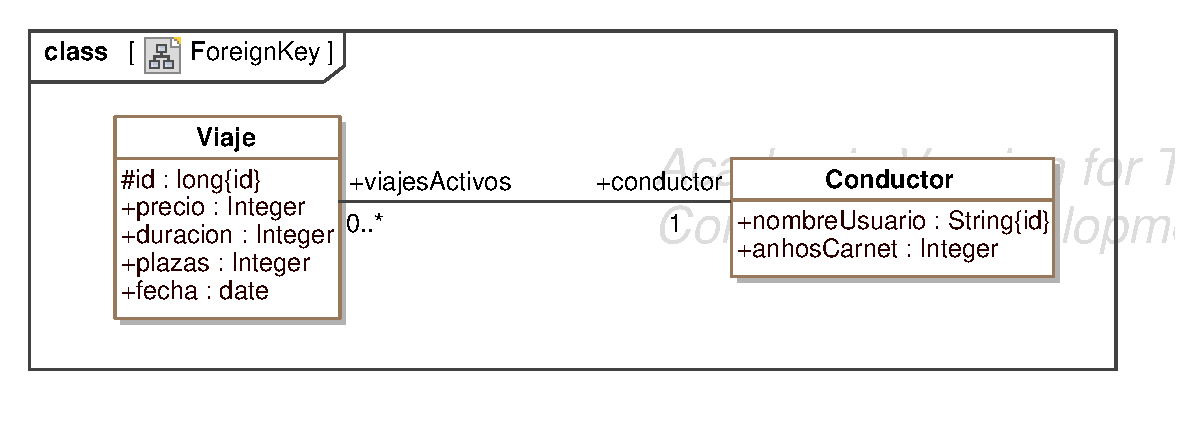
\includegraphics[width=0.75\linewidth]{images/structure/foreignKey00.eps}
%    }
%    \only<2->{
%        \rput[lt](2.25,-3.5){
%                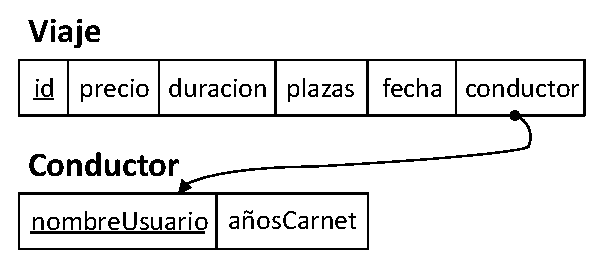
\includegraphics[width=0.60\linewidth]{images/structure/foreignKey01.eps}
%        }
%    }
%\end{frame}

%\subsection{Association Table Mapping}
%
%\begin{frame}[c]
%    \frametitle{Association Table Mapping}
%    \begin{block}{Problema}
%        ¿Cómo transformo una asociación entre clases al modelo relacional?
%    \end{block}
%    \uncover<2->{
%        \begin{block}{Solución}
%            \begin{enumerate}
%                \item<2-> Si ambos extremos de asociación tiene multiplicidad superior a uno, crear una tabla intermedia $A\_B$ que almacene la relación entre ambas clases.
%                \item<3-> La tabla intermedia almacenará como datos las claves primarias asociadas a las clases $A$ y $B$.
%                \item<4-> Cada una de estas claves primarias almacenadas será una clave externa a su correspondiente tabla.
%                \item<5-> La clave primaria de la tabla intermedia será la unión de las claves primarias de las tablas relacionadas.
%             \end{enumerate}
%        \end{block}
%    }
%\end{frame}
%
%\begin{frame}
%    \frametitle{Association Table Mapping}
%    \rput[lt](1.25,0.5){
%            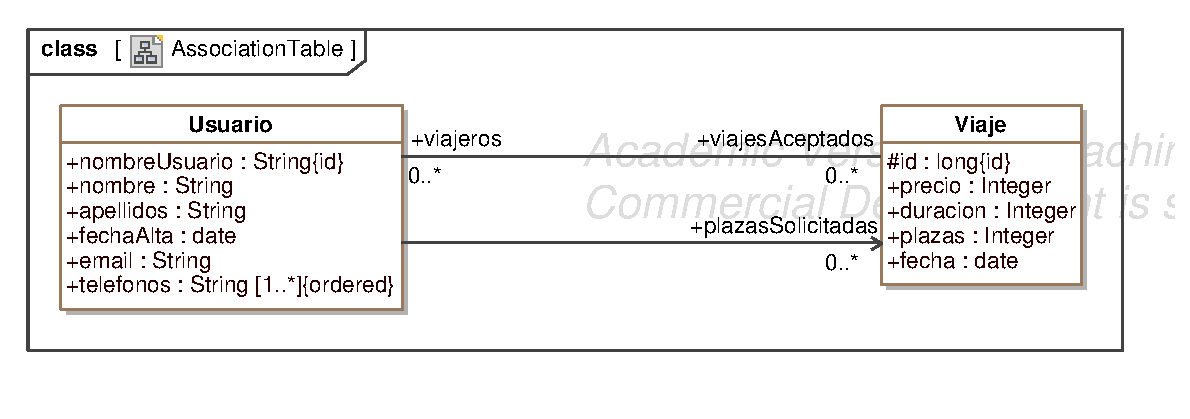
\includegraphics[width=0.80\linewidth]{images/structure/associationTable00.eps}
%    }
%    \only<2->{
%        \rput[lt](0.85,-3){
%                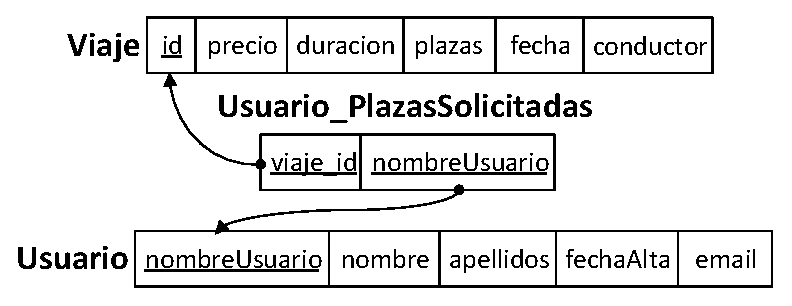
\includegraphics[width=0.75\linewidth]{images/structure/associationTable01.eps}
%        }
%    }
%\end{frame}

%\subsection{Embedded Value}
%
%\begin{frame}[c]
%    \frametitle{Embedded Value}
%    \begin{block}{Problema}
%        ¿Cómo mapeo asociaciones con \emph{value objects} de manera eficiente?
%    \end{block}
%    \uncover<3->{
%        \begin{block}{Solución}
%            Si una clase $C$ tiene una asociación de multiplicidad máxima $1$ con un \emph{value object } $V$, puedo simplemente añadir los campos de $V$ a la clase $C$ y luego mapear $C$ como una clase simple.
%        \end{block}
%    }
%\end{frame}

%\begin{frame}
%    \frametitle{Embedded Value}
%    \only<1|handout:1>{
%        \rput[lt](3.25,0){
%                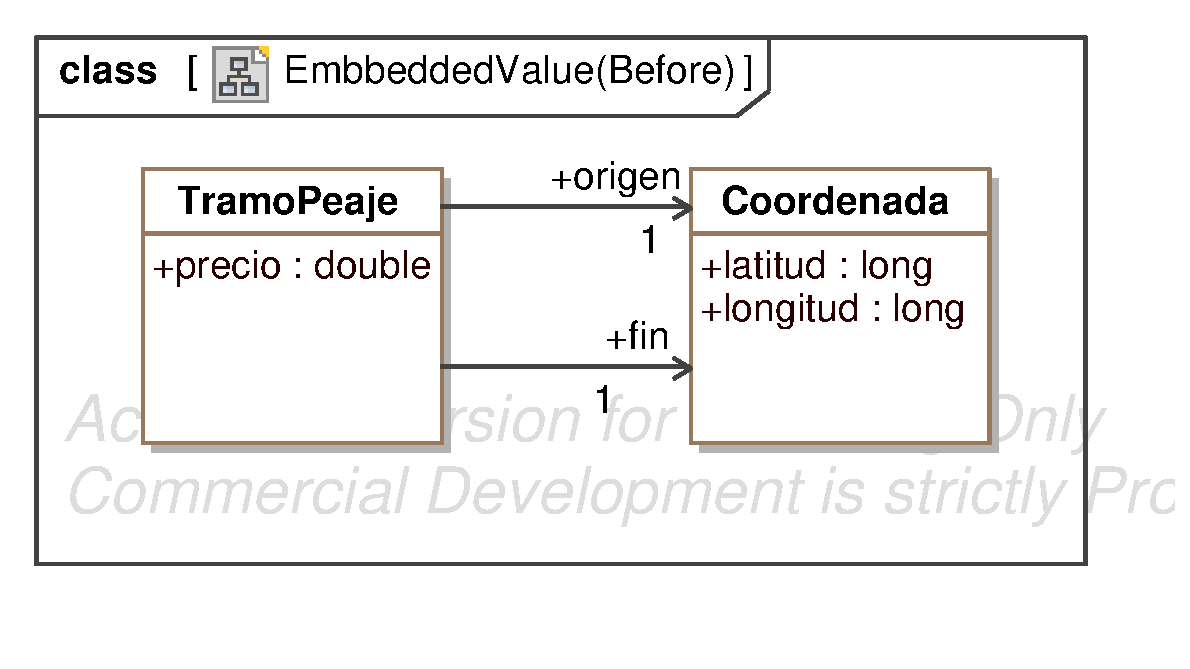
\includegraphics[width=0.50\linewidth]{images/structure/embeddedValue00.eps}
%        }
%    }
%    \only<2-|handout:0>{
%        \rput[lt](3.2,0){
%                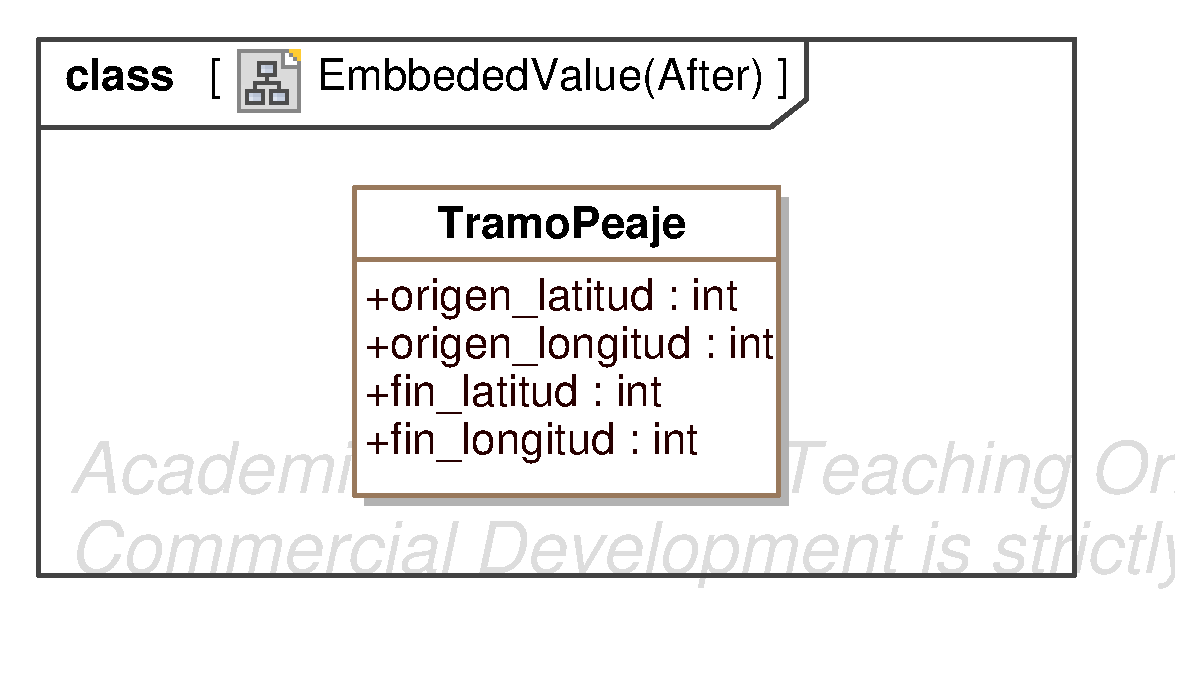
\includegraphics[width=0.50\linewidth]{images/structure/embeddedValue01.eps}
%        }
%    }
%    \only<3-|handout:1>{
%        \rput[lt](1,-4){
%                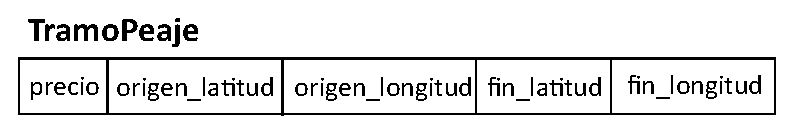
\includegraphics[width=0.75\linewidth]{images/structure/embeddedValue02.eps}
%        }
%    }
%\end{frame}

\subsection{Serialised Lob}

\begin{frame}[c]
    \frametitle{Serialised Blob}
    \begin{block}{Problema}
        ¿Cómo mapeo asociaciones con \emph{value objects} y/o \emph{entities} internas a un \emph{aggregate} de manera eficiente?
    \end{block}
    \uncover<3->{
        \begin{block}{Solución}
            Guardar todo un grafo de objetos en una única columna de tipo \emph{LOB}.
        \end{block}
    }
\end{frame}

\begin{frame}
    \frametitle{Serialised Blob}
    \rput[lt](1.50,0){
        \includegraphics[width=0.75\linewidth]{images/structure/serializedBlob00.eps}
    }
    \only<2->{
        \rput[lt](4.5,-3){
                \includegraphics[width=0.18\linewidth]{images/structure/serializedBlob01.eps}
        }
    }
    %% BLOB vs CLOB
\end{frame}

%\subsection{Single Table Inheritance}
%
%\begin{frame}[c]
%    \frametitle{Single Table Inheritance}
%    \begin{block}{Problema}
%        \begin{enumerate}
%            \item ¿Cómo transformo una jerarquía de herencia en un esquema relacional?
%        \end{enumerate}
%    \end{block}
%    \uncover<2->{
%        \begin{block}{Solución}
%            \begin{enumerate}
%                \item<2-> Comprimir la jerarquía en una sola clase, incorporando los atributos de las clases hijas a la raíz de la jerarquía.
%                \item<3-> Añadir un atributo que indique de qué tipo concreto es cada instancia de la nueva clase resultante.
%                \item<3-> Transforma la clase resultante a una tabla.
%                \item<4-> Cuando un objeto de dicha jerarquía se almacena dentro de la tabla resultante, los atributos que no correspondan a dicha instance simplemente se ignoran.
%            \end{enumerate}
%        \end{block}
%    }
%\end{frame}
%
%\begin{frame}
%    \frametitle{Single Table Inheritance}
%    \rput[lt](3.5,0){
%            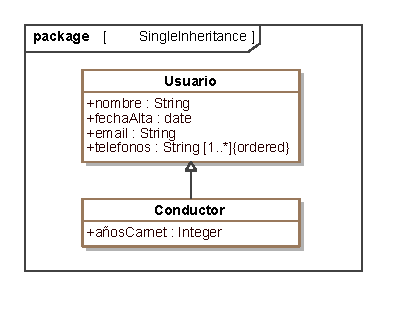
\includegraphics[width=0.50\linewidth]{images/structure/singleTable00.eps}
%    }
%%    \only<2->{
%%%        \rput[lt](3,-4){
%%%                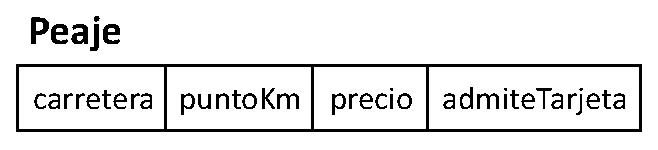
\includegraphics[width=0.50\linewidth]{images/structure/class2Table01.eps}
%%%        }
%%    }
%\end{frame}

\subsubsection{Concrete Table Inheritance}

\subsubsection{Class Table Inheritance}

\subsubsection{Comparación de Transformación de Herencias}

\section{Patrones de Acceso a Datos}

\subsubsection{Data Access Object}

\subsubsection{Metadata Mapping}

\subsection{Patrones Auxiliares}

\subsubsection{Lazy Load}

\subsubsection{Identity Map}

\subsubsection{Query Object}

%\subsubsection{Unit of Work}
%
%\begin{frame}[c]
%    \frametitle{Unit of Work - Problema}
%    \begin{block}{Problema}
%        Dentro de una misma \emph{transacción de negocio} se podrían realizar múltiples cambios en diversos objetos de dominio, por lo que estos cambios han de realizarse de manera transaccional.
%        \begin{emumerate}
%            \item<2-> Para poder gestionar la transacción, necesito saber con exactitud que ha cambiado, lo cual puede ser no trivial en ciertos casos (e.g., observadores).
%            \item<3-> Si cada cambio se refleja automáticamente en el sistema de persistencia, se generan demasiadas comunicaciones de pequeño tamaño, alguna de las cuales podría ser incluso no necesaria .
%            \item<4-> Necesito saber qué datos se han utilizado a lo largo de la transacción para poder determinar si dicha transacción es válida o no antes de confirmarla y cerrarla.
%        \end{emumerate}
%    \end{block}
%    %% Añadir una transparencia con un bloque de código.
%\end{frame}

%\begin{frame}[c]
%    \frametitle{Unit of Work - Solución}
%    \begin{block}{Solución}
%        \begin{enumerate}
%           \item<1-> Crear una clase denominada \emph{Unit of Work} donde se vayan registrando todos los cambios que se realizan dentro de una \emph{transacción de negocio}.
%           \item<2-> Hacer que los objetos de dominio cuando cambien se registren dentro de la unidad de trabajo como cambiados.
%           \item<3-> Hacer que los objetos de dominio utilizados dentro de una transacción se almacenen dentro de la unidad de trabajo como leídos.
%           \item<4-> Añadir métodos a la unidad de trabajo para validar y cerrar la transacción.
%       \end{enumerate}
%    \end{block}
%
%    %% Añadir imagen UML de Unit of Work.
%\end{frame}

%\section{Patrones de Control de la Concurrencia}
%
%\subsection{Pessimistic Lock}
%
%\begin{frame}[c]
%    \frametitle{Pessimistic Lock - Problema}
%    \begin{block}{Problema}
%        Cómo evitar conflictos cuando se accede a un mismo conjunto de datos de manera concurrente.
%    \end{block}
%    %% Poner escenario ilustrando el problema
%\end{frame}
%
%\begin{frame}[c]
%    \frametitle{Pessimistic Lock - Solución}
%    \begin{block}{Solución}
%        \begin{enumerate}
%           Cada transacción bloquea los datos que necesita de manera que otras transacciones no puedan hacer uso de ellos.
%       \end{enumerate}
%    \end{block}
%\end{frame}
%
%\subsection{Optimistic Lock}
%
%\begin{frame}[c]
%    \frametitle{Optimistic Lock - Problema}
%    \begin{block}{Problema}
%        Cómo evitar conflictos cuando se accede a un mismo conjunto de datos de manera concurrente.
%    \end{block}
%    %% Poner escenario ilustrando el problema
%\end{frame}
%
%\begin{frame}[c]
%    \frametitle{Optimistic - Solución}
%    \begin{block}{Solución}
%        \begin{enumerate}
%           Permito lecturas concurrentes y antes de guardar los datos compruebo que los datos que he utilizado no han sido modificados por otra transacción. Si hubiesen sido modificados, aborto la transacción.
%       \end{enumerate}
%    \end{block}
%\end{frame}

\section{Java Persistence API y Spring Data}

\subsection{Esquema}

\subsection{Anotaciones JPA}

\begin{frame}[c]
    \frametitle{Anotaciones JPA}
    \begin{description}
        \item[@Entity]
        \item[@Embeddable]
        \item[@Id]
        \item[@GeneratedValue]
        \item[@Embedded]
        \item[@OneToOne]
        \item[@OneToMany]
        \item[@ManyToOne]
        \item[@ManyToMany]
        \item[mappeddBy]
        \item[@Inheritance(strategy=)]
    \end{description}
\end{frame}

\begin{frame}[c]
    \frametitle{Ciclo de Vida de una Entidad JPA}
    %% Diagrama de las actividades
    %% Se puede llegar a través de agregados, es decir, como referencia desde
    %% una entidad, normalmente un agregado
\end{frame}

\begin{frame}[c]
    \frametitle{Ciclo de Vida de una Entidad JPA}
    %% Detecta transacciones de usuario.
\end{frame}

% \subsection{Validación en JPA}

\subsection{Clases JPA}

\subsection{Spring Data}

\section{Sumario y Conclusiones}

\end{document}
